\documentclass[12pt,a4paper]{article}

% ------------------------------
% Paquetes para idioma y tipografía
% ------------------------------
\usepackage[spanish]{babel}
\usepackage[utf8]{inputenc}
\usepackage[T1]{fontenc}
\usepackage{microtype}

% ------------------------------
% Paquetes para formato y gráficos
% ------------------------------
\usepackage{geometry}
\geometry{top=2.5cm,bottom=2.5cm,left=3cm,right=3cm}
\usepackage{graphicx}
\usepackage{setspace}
\usepackage{booktabs}
\usepackage{array}
\usepackage{hyperref}
\usepackage{url}
\usepackage{enumitem}
\usepackage{titlesec}
\usepackage{parskip}

% Formato de secciones
\titleformat{\section}{\large\bfseries}{}{0em}{}[\titlerule]
\titleformat{\subsection}{\normalsize\bfseries}{}{0em}{}

\begin{document}

% ==========================================
% PORTADA
% ==========================================
\begin{titlepage}
    \centering

    % Logos y texto institucional
    \begin{minipage}{0.25\textwidth}
        \centering
        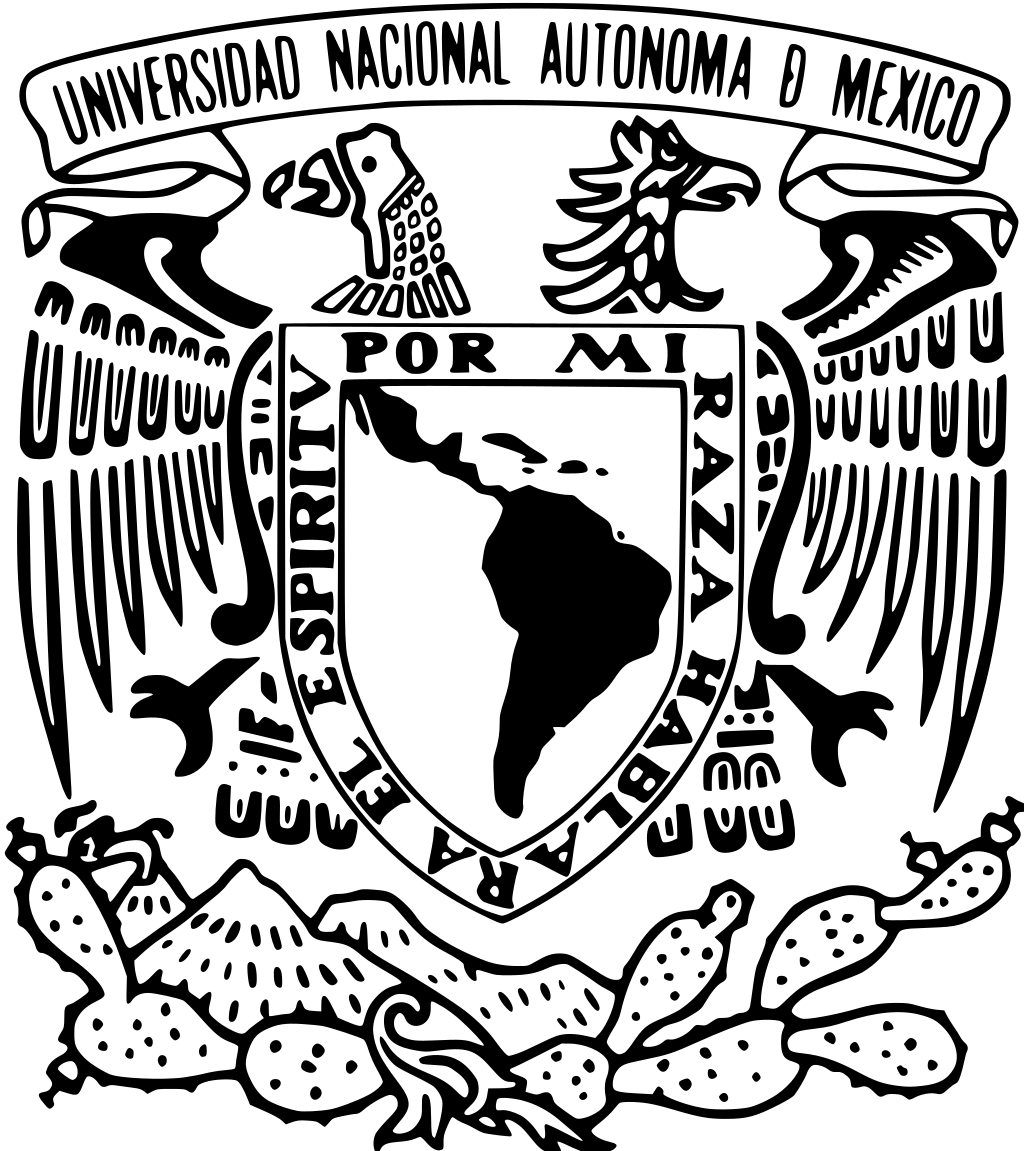
\includegraphics[width=3cm]{Escudo-UNAM.png}
    \end{minipage}
    \hfill
    \begin{minipage}{0.4\textwidth}
        \centering
        \textbf{\LARGE UNIVERSIDAD} \\[0.3cm]
        \textbf{\LARGE NACIONAL} \\[0.3cm]
        \textbf{\LARGE AUTÓNOMA} \\[0.3cm]
        \textbf{\LARGE DE MÉXICO} \\
    \end{minipage}
    \hfill
    \begin{minipage}{0.25\textwidth}
        \centering
        
\includegraphics[width=3cm]{escudofi_negro.jpg}
    \end{minipage}
    \\[0.75cm]
    {\large\textbf{FACULTAD DE INGENIERÍA}}\\[2cm]

    {\Large\textbf{AnteProyecto}}\\[0.5cm]
    {\large\textbf{Minería de Datos}}\\[0.5cm]
    {\large\textbf{Grupo: 1}}\\[2cm]

    \textbf{Equipo:}\\[0.3cm]
    Rojas Chimal Karla Beatriz \quad -- \quad 320048025\\[0.2cm]
    García Gallegos Alejandro \quad -- \quad 423093137\\[1.5cm]

    \textbf{Profesor:} Mtro. Gerardo Gabriel Carrasco Zúñiga\\[1.5cm]

    \textbf{Semestre:} 2027-1\\[2cm]
    \textbf{Fecha de entrega:} \today\\[1cm]

    \vfill
\end{titlepage}

\spacing{1.5}
\newpage

% ==========================================
% TABLA DE CONTENIDO
% ==========================================
\tableofcontents
\newpage

% ==========================================
% 1. OBJETIVOS
% ==========================================
\section{Objetivos}

\subsection{Objetivo General}
Desarrollar un modelo de clasificación binaria basado en técnicas de minería de datos para predecir
la probabilidad de que un paciente sufra un evento cerebrovascular (\textit{stroke}), a partir de
características clínicas y sociodemográficas disponibles en atención primaria.

\subsection{Objetivos Específicos}
\begin{itemize}[leftmargin=1.5cm]
    \item Analizar y preprocesar el \textit{Stroke Prediction Dataset} (5\,110 registros, 12 variables),
          identificando valores faltantes, distribuciones y desbalance de clases.
    \item Identificar las variables clínicas con mayor poder predictivo mediante análisis exploratorio
          de datos y técnicas de selección de características.
    \item Comparar el desempeño de al menos dos modelos de clasificación supervisada y seleccionar
          el más adecuado con base en métricas orientadas al contexto médico (AUC-ROC, \textit{recall}).
\end{itemize}

% ==========================================
% 2. CONTEXTO
% ==========================================
\section{Contexto}

\subsection{Descripción del Dominio}
Según la Organización Mundial de la Salud (OMS), el \textit{stroke} o evento cerebrovascular es la
segunda causa de muerte a nivel mundial, responsable de aproximadamente el 11\% del total de
defunciones. Se produce cuando el suministro de sangre al cerebro se interrumpe o se reduce,
privando al tejido cerebral de oxígeno y nutrientes.

La detección temprana de pacientes con alto riesgo permite diseñar intervenciones preventivas
oportunas, reduciendo la mortalidad y las secuelas neurológicas. Este proyecto aplica técnicas de
minería de datos sobre registros clínicos para construir un modelo predictivo que apoye la toma de
decisiones en el ámbito de la salud pública.

\subsection{Descripción del Dataset}
El conjunto de datos utilizado es el \textbf{Stroke Prediction Dataset}, publicado en Kaggle por
\textit{fedesoriano} (fuente confidencial, uso exclusivamente educativo). Contiene 5\,110
observaciones de pacientes, con 12 atributos clínicos y sociodemográficos.

Las variables disponibles son: \texttt{id} (identificador único), \texttt{gender}
(género: Male/Female/Other), \texttt{age} (edad en años), \texttt{hypertension} (0/1),
\texttt{heart\_disease} (0/1), \texttt{ever\_married} (Yes/No), \texttt{work\_type}
(Private/Self-employed/Govt\_job/children/Never\_worked), \texttt{Residence\_type} (Urban/Rural),
\texttt{avg\_glucose\_level} (glucosa promedio en sangre), \texttt{bmi} (índice de masa corporal)
y \texttt{smoking\_status} (formerly smoked/never smoked/smokes/Unknown). La variable objetivo es
\texttt{stroke} (1 = tuvo un stroke, 0 = no lo tuvo).

Observaciones relevantes sobre la calidad de los datos:
\begin{itemize}[leftmargin=1.5cm]
    \item La variable \texttt{bmi} presenta aproximadamente un 4\% de valores faltantes (\texttt{N/A}).
    \item La categoría \texttt{Unknown} en \texttt{smoking\_status} indica información no disponible
          para ese paciente.
    \item El dataset es significativamente desbalanceado: solo $\approx$9.8\% de los registros
          corresponden a casos positivos (498 strokes frente a 4\,612 no-strokes).
\end{itemize}

\begin{table}[h!]
\centering
\caption{Resumen del dataset}
\begin{tabular}{@{}lp{8cm}@{}}
\toprule
\textbf{Característica} & \textbf{Descripción} \\ \midrule
Fuente              & Kaggle --- fedesoriano (\textit{Stroke Prediction Dataset}) \\
No.\ de registros   & 5\,110 \\
No.\ de variables   & 12 (11 predictoras + 1 variable objetivo) \\
Periodo             & No especificado (uso educativo) \\
Variable objetivo   & \texttt{stroke} (binaria: 0 = no stroke, 1 = stroke) \\ \bottomrule
\end{tabular}
\end{table}

% ==========================================
% 3. ESTRATEGIA
% ==========================================
\section{Estrategia}

Se adoptará un enfoque de \textbf{clasificación supervisada binaria}, dado que la variable objetivo
(\texttt{stroke}) es discreta y etiquetada. La metodología de referencia será \textbf{CRISP-DM}
(\textit{Cross-Industry Standard Process for Data Mining}), que proporciona un marco iterativo
estructurado en seis fases.

Dado el marcado desbalance de clases (proporción $\approx$1:9), la estrategia incorporará técnicas
de manejo de desbalance como \textbf{SMOTE} (\textit{Synthetic Minority Oversampling Technique}) o
ajuste del parámetro \texttt{class\_weight} en los clasificadores. El criterio principal de éxito
será maximizar el \textbf{AUC-ROC} y el \textbf{recall} de la clase positiva, priorizando la
sensibilidad del modelo sobre la precisión, lo cual es más relevante en contextos de diagnóstico
médico.

\subsection{Fases del Proyecto}
\begin{enumerate}[leftmargin=1.5cm]
    \item \textbf{Recolección y comprensión de datos:} Descarga del dataset desde Kaggle mediante
          \texttt{kagglehub}, revisión de atributos, tipos de datos, distribuciones iniciales y
          detección de anomalías.
    \item \textbf{Preprocesamiento y limpieza:} Imputación de valores faltantes en \texttt{bmi},
          codificación de variables categóricas (\textit{one-hot encoding}), tratamiento del
          desbalance de clases y normalización de variables numéricas.
    \item \textbf{Exploración y análisis:} Análisis exploratorio de datos (EDA): distribuciones,
          correlaciones, análisis bivariado respecto a la variable objetivo y visualización de
          patrones relevantes.
    \item \textbf{Modelado:} Entrenamiento y ajuste de al menos dos clasificadores (e.g.,
          Regresión Logística y Random Forest) con validación cruzada estratificada
          (\textit{k-fold}).
    \item \textbf{Evaluación y refinamiento:} Comparación de modelos mediante AUC-ROC, F1-score
          y recall. Análisis de la matriz de confusión y curvas ROC. Selección del modelo final.
    \item \textbf{Presentación de resultados:} Elaboración del reporte final y demostración
          técnica en notebook interactivo.
\end{enumerate}

% ==========================================
% 4. PROBLEMÁTICA A ATENDER (EXPECTATIVAS)
% ==========================================
\section{Problemática a Atender y Expectativas}

\subsection{Planteamiento del Problema}
El \textit{stroke} es una emergencia médica cuyo pronóstico mejora significativamente con la
intervención temprana. Sin embargo, muchos pacientes en riesgo no son identificados a tiempo por
la falta de herramientas de cribado accesibles en atención primaria. Los registros clínicos
electrónicos contienen información valiosa que, analizada con técnicas de minería de datos, puede
transformarse en un sistema de alerta temprana.

El problema central es: \textbf{¿Es posible predecir con suficiente sensibilidad si un paciente
sufrirá un stroke, utilizando únicamente variables clínicas y demográficas de rutina?} La respuesta
a esta pregunta permitirá orientar acciones preventivas y optimizar la asignación de recursos
médicos.

\subsection{Preguntas de Investigación}
\begin{itemize}[leftmargin=1.5cm]
    \item ¿Qué combinación de variables clínicas (edad, hipertensión, glucosa, IMC, etc.) es más
          predictiva de un evento cerebrovascular?
    \item ¿Qué modelo de clasificación supervisada ofrece el mejor equilibrio entre sensibilidad
          (\textit{recall}) y precisión en este dataset desbalanceado?
    \item ¿Cómo afecta el tratamiento del desbalance de clases (SMOTE vs.\ sin tratamiento) al
          desempeño de los modelos evaluados?
\end{itemize}

\subsection{Expectativas}
Se espera que el modelo final alcance las siguientes métricas sobre el conjunto de prueba:

\begin{itemize}[leftmargin=1.5cm]
    \item \textbf{AUC-ROC $>$ 0.85:} indicador global de capacidad discriminativa del modelo.
    \item \textbf{Recall (clase positiva) $>$ 0.75:} prioritario en contexto médico para minimizar
          falsos negativos (pacientes en riesgo no detectados).
    \item \textbf{F1-score $>$ 0.60:} balance entre precisión y recall, considerando el desbalance
          de clases.
\end{itemize}

Cualitativamente, se espera identificar las variables con mayor influencia en la predicción
(\texttt{age}, \texttt{avg\_glucose\_level} e \texttt{hypertension} se anticipan como las más
relevantes según literatura), y generar visualizaciones que comuniquen los hallazgos de forma clara.

% ==========================================
% 5. PLAN DE TRABAJO: BASELINE VS. REAL
% ==========================================
\section{Plan de Trabajo: Baseline vs.\ Real}

\subsection{Plan Baseline}
El plan inicial contempla un desarrollo de cuatro semanas, distribuido de la siguiente forma:

\begin{itemize}[leftmargin=1.5cm]
    \item \textbf{Semana 1:} Descarga y familiarización con el dataset. Revisión bibliográfica sobre
          predicción de stroke. Definición del alcance y reparto de tareas entre los integrantes.
    \item \textbf{Semana 2:} Preprocesamiento completo (imputación, codificación, manejo de
          desbalance) y análisis exploratorio de datos.
    \item \textbf{Semana 3:} Entrenamiento, ajuste y comparación de modelos de clasificación.
    \item \textbf{Semana 4:} Evaluación final, elaboración del reporte y preparación de la
          demostración.
\end{itemize}

\subsection{Plan Real}
\textit{[Por completar al finalizar el proyecto. Se documentarán aquí los ajustes realizados
respecto al plan baseline, incluyendo retrasos, tareas no contempladas y su justificación.]}

\subsection{Tabla Comparativa}
\begin{table}[h!]
\centering
\caption{Comparación Plan Baseline vs.\ Real}
\begin{tabular}{@{}p{4cm}p{4.5cm}p{4.5cm}@{}}
\toprule
\textbf{Actividad} & \textbf{Baseline} & \textbf{Real} \\ \midrule
Recolección de datos    & Semana 1       & \textit{[Por completar]} \\
Preprocesamiento        & Semana 2       & \textit{[Por completar]} \\
Análisis exploratorio   & Semana 2       & \textit{[Por completar]} \\
Modelado                & Semana 3       & \textit{[Por completar]} \\
Evaluación              & Semanas 3--4   & \textit{[Por completar]} \\
Redacción del reporte   & Semana 4       & \textit{[Por completar]} \\ \bottomrule
\end{tabular}
\end{table}

% ==========================================
% 6. METODOLOGÍA APLICADA
% ==========================================
\section{Metodología Aplicada}

\textit{[Por completar. Describir la metodología de modelado aplicada. Indicar si se siguió
CRISP-DM u otro marco. Especificar modelos, justificación, estrategia de validación y criterio
de selección del modelo final.]}

\subsection{Preprocesamiento}
\textit{[Por completar. Describir el tratamiento de valores faltantes, codificación de variables
categóricas, normalización/estandarización, detección de outliers y cualquier transformación
aplicada.]}

\subsection{Modelos Considerados}
\begin{itemize}[leftmargin=1.5cm]
    \item \textbf{Modelo 1:} \textit{[nombre y justificación]}
    \item \textbf{Modelo 2:} \textit{[nombre y justificación]}
    \item \textbf{Modelo 3 (opcional):} \textit{[nombre y justificación]}
\end{itemize}

\subsection{Validación y Métricas}
\textit{[Por completar. Indicar la estrategia de validación y las métricas de desempeño
utilizadas (AUC-ROC, F1-score, recall, matriz de confusión, etc.).]}

% ==========================================
% 7. HERRAMIENTAS DE MD APLICADAS Y RESULTADOS
% ==========================================
\section{Herramientas de Minería de Datos y Resultados}

\subsection{Herramientas Utilizadas}
\begin{itemize}[leftmargin=1.5cm]
    \item \textbf{Python 3.x:} entorno principal de desarrollo.
    \item \textbf{kagglehub:} descarga automatizada del dataset desde Kaggle.
    \item \textbf{Pandas / NumPy:} manipulación y análisis de datos.
    \item \textbf{Scikit-learn:} clasificadores, validación cruzada y métricas.
    \item \textbf{imbalanced-learn:} técnicas de manejo de desbalance (SMOTE).
    \item \textbf{Matplotlib / Seaborn:} visualización de datos y resultados.
\end{itemize}

\subsection{Resultados Obtenidos}
\textit{[Por completar. Presentar los resultados de cada modelo evaluado. Incluir tabla
comparativa de métricas, análisis de las curvas ROC y hallazgos del análisis exploratorio.]}

\begin{table}[h!]
\centering
\caption{Comparación de modelos}
\begin{tabular}{@{}lllll@{}}
\toprule
\textbf{Modelo} & \textbf{AUC-ROC} & \textbf{Recall} & \textbf{F1-score} & \textbf{Observaciones} \\ \midrule
\textit{Modelo 1} & -- & -- & -- & -- \\
\textit{Modelo 2} & -- & -- & -- & -- \\
\textit{Modelo 3} & -- & -- & -- & -- \\ \bottomrule
\end{tabular}
\end{table}

\subsection{Demo}
\textit{[Por completar. Describir la demostración técnica: tipo (notebook interactivo, script,
aplicación), qué permite visualizar o ejecutar y cómo reproducirla.]}

% ==========================================
% 8. CONCLUSIONES
% ==========================================
\section{Conclusiones}

\textit{[Por completar. Indicar si se alcanzaron los objetivos planteados, los principales
hallazgos, las limitaciones encontradas y las recomendaciones para trabajo futuro.]}

% ==========================================
% 9. FUENTES BIBLIOGRÁFICAS (APA)
% ==========================================
\section{Fuentes Bibliográficas}

\begin{itemize}[leftmargin=1.5cm, label={}]
    \item Organización Mundial de la Salud. (2023). \textit{Las 10 principales causas de defunción}.
          OMS. \url{https://www.who.int/es/news-room/fact-sheets/detail/the-top-10-causes-of-death}
    \item fedesoriano. (2021). \textit{Stroke Prediction Dataset} [Conjunto de datos]. Kaggle.
          \url{https://www.kaggle.com/datasets/fedesoriano/stroke-prediction-dataset}
    \item \textit{[Referencia 3 en formato APA 7.ª ed.]}
\end{itemize}

\end{document}
